\chapter{Introduction to Git}

This document is designed to provide a detailed outline of the correct way to contribute in Antonius' Handbook. This manual will outline the process of setting up git on a machine for tracking project changes, making properly formatted changes, and pushing changes to the git server. For a proper editing environment, Git and a \LaTeX editor are required. By the nature of this project, this tutorial will assume basic computer skills and knowledge.


\section{Installing Git}

Before additions can be made to Antonius' Handbook, you must have a way to obtain the current source code. This is done via Git by downloading and syncing the source code to the most recent copy before editing. All code for this project is open sourced on Github. Github is a site that allows storage of different projects that utilize git for pushing changes. This is useful because many users can simultaneously work on a single project, push changes to a single location, track changes, recover changes, and more. Github is free to use for any non-private repositories and also offers a paid service for private repositories that cannot be seen by public users. For the purposes of this tutorial, we will focus on the command line commands via Git.

\begin{enumerate}
	\item Head over to https://git-scm.com/ and download the latest release. See figure \ref{git}. 
	
	\begin{figure}[h]
		\centering
		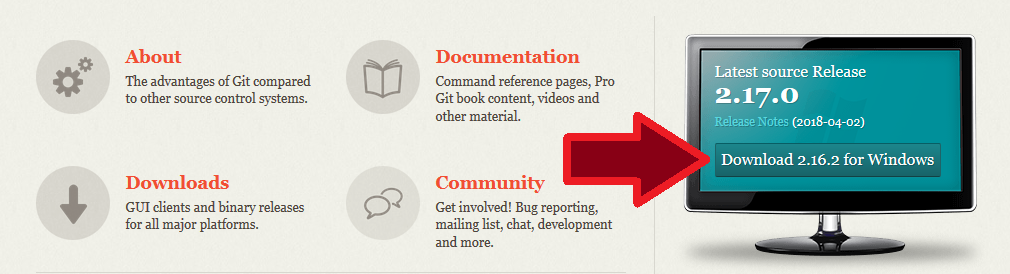
\includegraphics[width=0.8\textwidth]{images/git.png}
		\caption{Git download from the git-scm homepage.} \label{git}
	\end{figure}

	\item Install Git using the latest release launcher. This will vary depending on your operating system. Installing Git using the recommended settings should be sufficient.
\end{enumerate}


\section{Obtaining Project Source}

Once you have Git installed you are ready to retrieve the project source code you are working with. For the purposes of this tutorial we will use Antonius' Handbook (AH) Volume II as an example. 

\begin{enumerate}
	\item First, you will need to obtain the URL to the project. For a project like AH, this can be found on the homepage of the project via the "clone or download" button. See figure \ref{gitclone}.
	
	\begin{figure}[h]
		\centering
		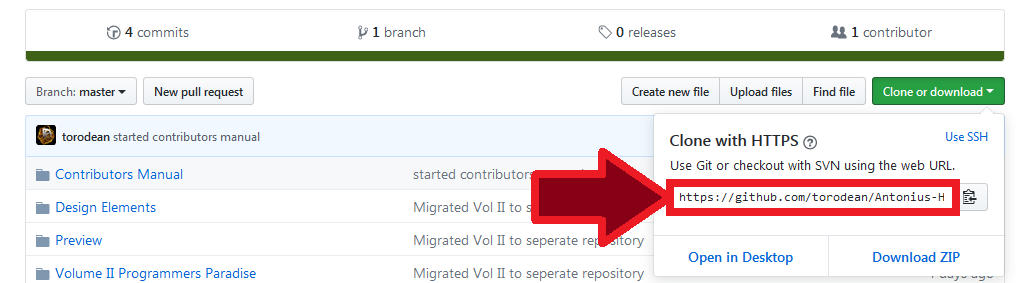
\includegraphics[width=0.8\textwidth]{images/gitclone.png}
		\caption{Link to the Github project.} \label{gitclone}
	\end{figure}

	\item Next, you will need to open a command prompt (if you're on Windows), terminal (For Linux and Mac users), or the git gui (if you know how to use it) and navigate to the directory where you want to save the source files. To change directory in the Windows command prompt or Linux terminal use the commands below.
	
\begin{lstlisting}
cd desired/directory/for/saving/files/
\end{lstlisting}
	
	\item Next, you will need to clone the project source to your computer by using the git clone command. This is done by entering "git clone" followed by the url that we acquired in the previous step.
	
\begin{lstlisting}
git clone https://github.com/torodean/Antonius-Handbook-II.git
\end{lstlisting}
\end{enumerate}

Once you have completed the above steps you are ready to make changes and use the source files you've acquired!



\section{Making Changes and Saving Them Through Git}

Once you've acquired the source files, you can edit and modify them through any means you like. Git will automatically track any changes that are made within the project directory that you acquired through git clone. However, this does not mean that git will save all changes to the server automatically. There are no limitations (for normal editing and file usage) as to what can be done within this folder, however, in order to avoid conflicts, there are a few things that should be considered while making edits.

\begin{enumerate}
	\item When making changes to a Git repository shared between users, if one person has un-pushed (meaning saved to the server) changes while the other is editing files, this can cause conflicts. 
	\item Before editing any files in the directory, it is important to make sure you have the most up to date files. This is done through the following command while in the project directory.
	
\begin{lstlisting}
git pull
\end{lstlisting}

	\item You can view the status of whether you have made changes to a repository since pulling it via the following command.
	
\begin{lstlisting}
git status
\end{lstlisting}

	\item Depending on the user interface you are interfacing through git, you will see different changes to the directory. Through a terminal view, if there are untracked changes, you will see the changed files and folder in red. In order to add changes to the server, you must first tell Git you want to add those changes. This is done via the following command.
	
\begin{lstlisting}
git add <FILES>        # Use this to add single files/folders.
git add -A             # Use this command to add all changes.
\end{lstlisting}

	\item After adding file changes, they should now appear in green after running 'git status'. The next step is to tell Git that you would like to commit those changes. At the same time of committing the changes, you cn add a message as to what the commit is (what was changed from the original repository). This is done via the following command.
	
\begin{lstlisting}
git commit -m "Message describing what we are changing"
\end{lstlisting}

	\item Now all that's left is to finalize the changes to the server by running the following command. This will push all changes to the server.
	
\begin{lstlisting}
git push
\end{lstlisting}
	
\end{enumerate}


\section{Resetting and Restoring A project}

In some cases, mistakes are made and files are deleted by accident. By default, git will not let you simple "git pull" to restore files. This is because Git has no way of knowing whether the file deletions were intentional. In cases where major mistakes or errors have been made in a repository, it is best to either delete the repository and re-clone it, or run the following command

\begin{lstlisting}
# Use this command carefully as it will remove all non-pushed cahnges.
git reset --hard
\end{lstlisting}



\chapter{Installing and Using LaTeX}

This section is relevant for users wanting to edit source projects pertaining to the user of \LaTeX. 

\section{Installing MiKTeX}

MiKTeX is implementation of TeX/\LaTeX that is kept up to date. To install MiKTeX, please head to https://miktex.org/ and following the instructions that exist there.

\section{Installing TeX Studio}

After installing MiKTeX, you will need to decide on which \LaTeX integrated development environment (IDE) you would like to use for editing \LaTeX documents. Personally, I have had great success with TeXstudio and thus will be using that throughout this tutorial. I would also recommend TeXstudio to anyone wanting to learn \LaTeX as it is easy to use and user friendly. To download this IDE, first head to https://www.texstudio.org/ and download the most recent version. See figure \ref{TeXstudio}. Then, run the installer. The default options upon install should be sufficient for using the program.

\begin{figure}[h]
	\centering
	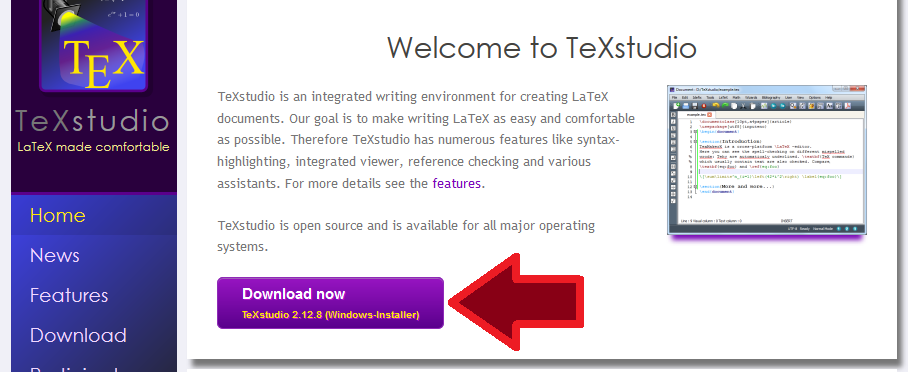
\includegraphics[width=0.8\textwidth]{images/texstudio.png}
	\caption{Download button for the TeXstudio IDE.} \label{TeXstudio}
\end{figure}


After downloading and installing TeXstudio, you are ready to edit \LaTeX files via TeXstudio! 


